\section{Methodology}

The robot that will be used is the adult-size humanoid robot Jaemi Hubo, see Fig.~\ref{fig:huboSch}.  Jaemi Hubo is a high gain position controlled device.  Each actuator is fed a reference position and is able to feed back the actual position, the current through the actuator, and the actuator status (enabled or disabled).  Each actuator has an over current automatic disable routine.  When this routine is executed the motor control is deactivated but feedback of the actual position is still enabled.

\begin{figure}[thpb]
  \centering
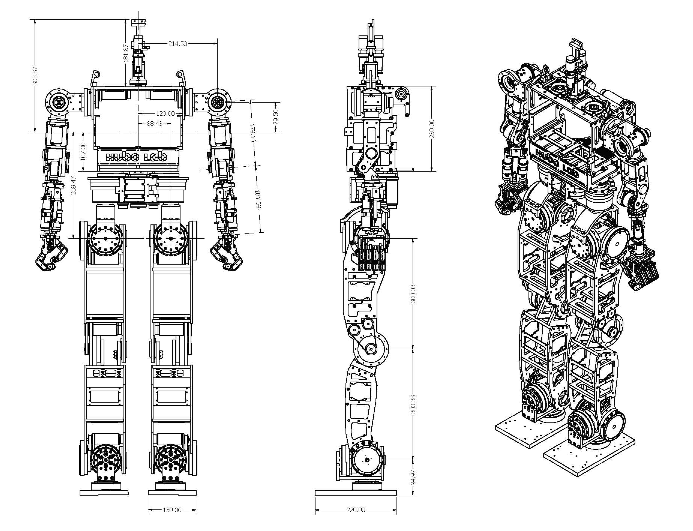
\includegraphics[width=1.0\columnwidth]{./pix/huboSch.png}
  \caption{Jaemi Hubo: 130cm tall 45kg (with battery and protective shell) 40 degree of freedom, high gain position controlled adult-size humanoid robot }
  \label{fig:huboSch}
\end{figure}